\section{Answer part one}
%Identify the stakeholders in your project and describe their interests in the project and  how you will handle them
\begin{center}
	\begin{tabular}[h]{|c|p{25em}|}
		\hline
		Stakeholder & Interest \\ \hline
		General Practitioners & They are our target demographic as they use the service to provide better healthcare to their clients. Developing our program will be able to increase the confidence of their diagnoses. \\ \hline
		Developers & They are interested in it because their business and thereby wages depends on it, delivering a good product could gain them good advantages when it comes to income and or future job prospects. \\ \hline
		Healthcare companies & The companies that hires the General Practitioners are the one who will most likely be paying for our service, their interested is whether this will earn them more revenue either in the long run or short term.\\ \hline
	\end{tabular}
\end{center}

%Create a WBS for your project and document it as a table
In this project, the group are using a Top-Down estimation process because of the following reasons:
\begin{itemize}
	\item It's the first time the group develops a project for healthcare and thereby don't know completely what is involved yet.
	\item It's a small project and the group only have two developers, the scope of the project is small.
	\item There is no contract involved.
	\item There is no current customer, only general practitioners who have offered to guide and therefore no details are needed for the customers.
\end{itemize}
For the development of the product, it is split up in 3 section in the WBS, Frontend, Backend and server. 
\begin{center}
	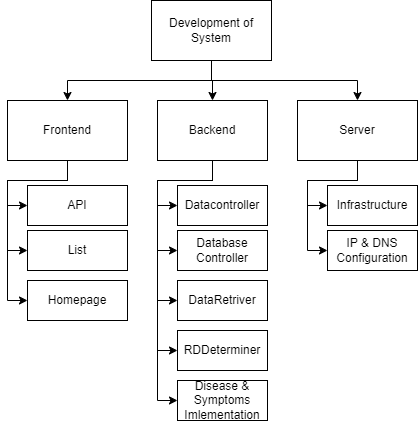
\includegraphics[width=.5\columnwidth]{./WBS}
\end{center}

\begin{center}
	\begin{tabular}[h]{|c|c|c|}
		\hline
		Task & Dependency & Estimated Time (hours) \\ \hline
		ISymptom & & \\ \hline
		Region & &  \\ \hline
		IDisease & &  \\ \hline
		Symptom & ISymptom, Region &  \\ \hline
		Disease & IDisease & \\ \hline
		DatabaseController & Disease, Symptom & \\ \hline
		DataController & DatabaseController &  \\ \hline
		DataRetriver & DatabaseController & \\ \hline
		IDeterminer & &  \\ \hline
		RDDeterminer & IDeterminer, DataRetriver & \\ \hline
		API & DataController & \\ \hline
		Homepage & & \\ \hline
		Infrastructure & & \\ \hline
		IP \& DNS & Homepage & \\ \hline
	\end{tabular}
\end{center}

Slut: 28.April
%Write a POS for your project using the template on p. 126 in Effective Project Management(Wysocki)
\begin{center}
	\begin{tabular}[h]{|p{7em}|p{5em}|p{5em}|p{5em}|p{5em}|}
		\hline
		& {\scriptsize Project Overview Statement} & {\scriptsize Rare disease Predictor} & & {\scriptsize Simon dos Reis Spedsbjerg} \\ \hline
		{\scriptsize Problem/Opportunity} & \multicolumn{4}{|p{20em}|}{\scriptsize We see a risk that a healthcare professional might miss certain rare conditions a patient might suffer from, because the rarity and lack of knowledge makes it so the doctor or nurse might not suspect it and thereby miss it.}\\ \hline
		{\scriptsize Goal} & \multicolumn{4}{|p{20em}|}{\scriptsize To develop an application that will help the health care professional to deduce whether a patient suffers from a rare disease}\\ \hline
		{\scriptsize Objectives} & \multicolumn{4}{|p{20em}|}{\scriptsize \begin{itemize}
		\item Develop a Backend system to calculate diseases based on symptoms
		\item Develop a Frontend to allow interaction from any computer
		\item Establish a server to host a beta version
		\item Deploy public version
			 \end{itemize}
		 } \\ \hline
	 {\scriptsize Success Criteria} & \multicolumn{4}{|p{20em}|}{\scriptsize\begin{itemize}
	 	\item The system can predict diseases based on given symptoms
	 	\item The system is positively received by general practitioners
	 	\item The system is being used by general practitioners
	 \end{itemize}} \\ \hline
 	{\scriptsize Assumptions, Risks, Obstacles} & \multicolumn{4}{|p{20em}|}{\scriptsize
 	\begin{itemize}
 		\item All general practitioners have access to the internet
 		\item Server Errors might occur
 		\item Some general practitioners don't have the required computer knowledge to use the system
 	\end{itemize}	
 }\\ \hline
& {\scriptsize Simon Spedsbjerg} & {\scriptsize $07-03-23$} & & \\ \hline
	\end{tabular}
\end{center}
%Identify the risks in the project, create a risk severity matrix, and explain how you will handle the risks

%Estimate the tasks in your WBS. Argue for the selection of estimation method

%Create a network diagram for your project and identify 1) the earliest finish date for theproject and 2) the critical path

%Create  a  short  presentation  that  you  can  use  in  class  to  present  your  results  to  othergroups


Read stuff from\cite{Larson2021}.